\section{焦耳定律}\label{sec:9-4}

从电流的热效应知道,当电流通过导体的时候,导体要发热。
这时电流做功,电能转化成热能,使导体和周围物体的温度升高。
因为这相当于传给导体和周围物体一定的热量,所以习惯上常把这种能量转化现象叫做电流产生了热量。

在工农业生产和日常生活中,有时要利用电流产生的热量,有时要减少这种热量。
因此,需要知道电流产生的热量跟哪些因素有关系。下面我们用实验来研究这个问题。

在甲、乙两个相同的瓶子里装满煤油,各放一根电阻丝(图 \ref{fig:9-5}),甲瓶中电阻丝的电阻比乙瓶中的大。
如果有电流通过电阻丝,电流产生的热量就使煤油温度升高,体积膨胀,在玻璃管内上升。
在同样时间里,电流产生的热量越多,煤油在玻璃管内上升得越高。
因此,注意观察玻璃管内煤油上升的情况,就可以比较电流通过这两根电阻丝产生的热量。

\begin{figure}[htbp]
    \centering
    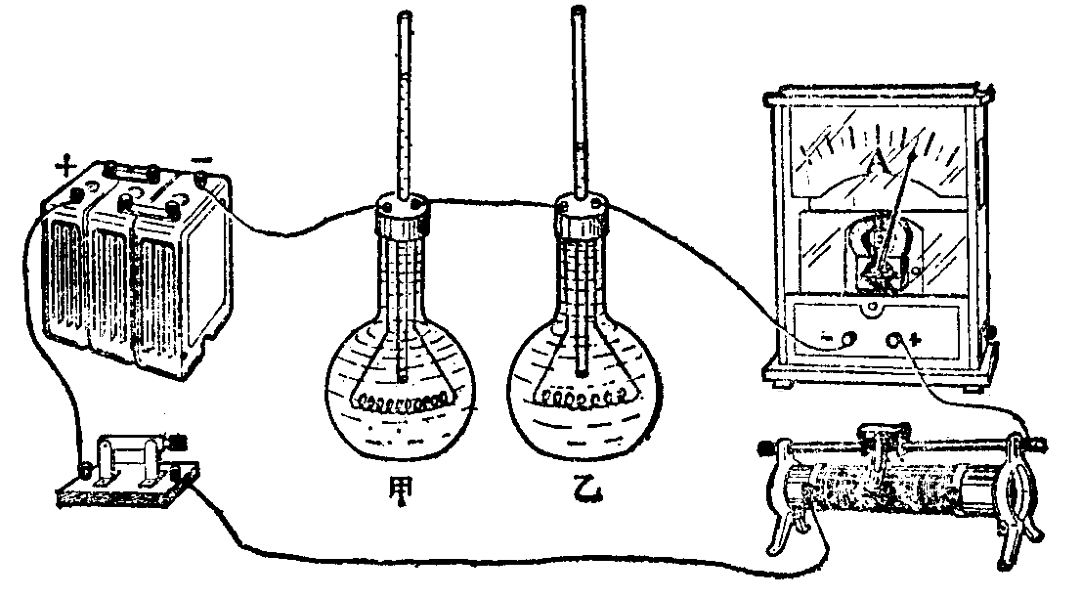
\includegraphics[width=0.8\textwidth]{../pic/czwl2-ch9-5}
    \caption{}\label{fig:9-5}
\end{figure}

照图 \ref{fig:9-5} 接通电路,可以看到甲瓶玻璃管中的煤油比乙瓶上升得高。
这两根电阻丝是串联着,电流强度和通电时间都相等,只是甲瓶电阻丝的电阻比乙瓶的大,
可见,\CJKunderwave{电阻越大,电流产生的热量越多}。

调节滑动变阻器,使电路中的电阻减小,然后闭合电键,使通电时间跟前次实验的相等。
可以看到电路中的电流强度变大,两管中的煤油都比前次实验上升得高。
比较一下这两次实验,我们会得到什么结论呢?
在这两次实验中,每根电阻丝的电阻并没有改变,通电时间又相等,只是第二次实验的电流强度大。
可见,\CJKunderwave{电流强度越大,电流产生的热量越多}。

在上面的两次实验里都可以看出,
\CJKunderwave{通电时间越长,电流产生的热量越多}。

英物理学家焦耳做了大量的实验,于 1840 年最先精确地确定了电流产生的热量跟电流强度、电阻和时间的关系:
\textbf{电流流过导体产生的热量,跟电流强度的平方成正比,跟导体的电阻成正比,跟通电的时间成正比}。
这个规律叫\textbf{焦耳定律}。

焦耳定律可以用下面的公式来表示:
$$ Q = I^2Rt \;\juhao $$

在这个公式中,电流强度 $I$ 的单位用安培,电阻 $R$ 的单位用欧姆,时间 $t$ 的单位用秒,
电流产生的热量 $Q$ 的单位用焦耳。

焦耳定律的公式也可以用我们学过的知识推导出来,如果电流通过金属导体时,电能全部转化成了热能,
而没有转化为其他形式的能,这时电流产生的热量就等于电流所做的功,即 $Q = W$。
电流所做的功 $W = UIt$,根据欧姆定律 $U = IR$,于是得到 $W = I^2Rt$。
由于 $Q = W$,因此 $Q = I^2Rt$,这就是焦耳定律。

\liti 某电热器接在 220 伏特的电源上,电阻是 55 欧姆,它 5 分钟产生多少热量?

在这个题目中,电路中的电流强度没有给出,因而要先由欧姆定律计算出电流强度,
再由焦耳定律公式计算电流产生的热量。

\begin{enhancedline}
解:$\begin{aligned}[t]
    &I = \dfrac{U}{R} = \dfrac{220\fute}{55\oumu} = 4\anpei \;\text{,} \\
    &Q = I^2Rt = (4\anpei)^2 \times 55\oumu \times 300\miao = 2.64 \times 10^5 \jiaoer \;\juhao
\end{aligned}$
\end{enhancedline}

答:这个电热器 5 分钟产生 $2.64 \times 10^5$ 焦耳的热量。

